\documentclass[a4paper]{article} % A4 paper and 11pt font size

\usepackage{braket}
\usepackage{amsmath}
\usepackage{amssymb}
\usepackage{bm}
\usepackage[utf8]{inputenc}
\usepackage{verbatim}
\usepackage{tikz}
%\usepackage{tikz-feynman}
\usepackage{pgfplots}
\usepackage{pgffor}
\usepackage[version-1-compatibility]{siunitx}
\usepackage{fancyhdr}
\usepackage{mathtools} %for underbraces without whitespace (\mathclap{})


\usepackage{hyperref}
\usepackage{geometry}

 \geometry{
 a4paper,
 total={210mm,297mm},
 left=28mm,
 right=28mm,
 top=30mm,
 bottom=40mm,
 }


\usepackage{framed}
\usepackage{amssymb} %for Lagrangian L, order O
\usepackage{cancel} %for strikethroughs
\usepackage{slashed} %for Feynman slashes

\newcommand{\pmx}[1]{\begin{pmatrix}#1\end{pmatrix}}
\newcommand{\ph}[1]{\phantom{#1}}

\usepackage{gensymb}

\usepackage{fancyhdr}
\usepackage{pdflscape}
\usepackage{bm}

%for side-by-side figures
\usepackage{graphicx}
\usepackage{caption}
\usepackage{subcaption}

\setlength{\parindent}{2em}
\setlength{\parskip}{1em}
\renewcommand{\baselinestretch}{1.1}


%----------------------------------------------------------------------------------------
%	TITLE SECTION
%----------------------------------------------------------------------------------------
\setlength\parindent{0pt} % Removes all indentation from paragraphs - comment this line for an assignment with lots of text


\pagenumbering{arabic}
\begin{document}
\pagestyle{empty}

\newcommand{\HRule}{\rule{\linewidth}{0.5mm}}

\begin{titlepage}

    \begin{center}
        \textsc{\large SN: 587623}\\[6cm]

        \HRule \\[0.5cm]
		\Huge \textbf{PHYC90012 General Relativity}\\[0.5cm]
        \huge \textbf{Assignment 2}\\[0.5cm] 
        \HRule \\[1.5cm]
        \begin{minipage}{0.4\textwidth}
        \begin{center}

        \large By \\[0.75cm]
        \huge Braden \scshape Moore \\[0.5cm]
        \normalsize \normalfont Master of Science \\
        The University of Melbourne \\

        \end{center}
        \end{minipage}

        \vfill

        \large \today
    \end{center}

\newpage
\end{titlepage}
%----------------------------------------------------------------------------------------
\pagestyle{fancy}
\pagenumbering{arabic}
\rfoot{\textsc{Braden Moore, 587623}}
\lfoot{\textsc{\today}}
\rhead{\textsc{General Relativity: Assignment 2}}
\setcounter{page}{1}
\setcounter{section}{1}
\section{Klein's geometry}
%%%%%%%%%%%%%%%%%%%%QUESTION 1%%%%%%%%%%%%%%%%%%%%%
\begin{framed}
A two-dimensional surface is covered by coordinates $(u,v)$ in the domain $u^2+v^2=1$. The independent components of the metric are given by
\begin{align}
g_{11}&=\frac{a^2(1-v^2)}{(1-u^2-v^2)^2},\label{1eq1}\\
g_{12}&=\frac{a^2 uv}{(1-u^2-v^2)^2},\\
g_{22}&=\frac{a^2(1-u^2)}{(1-u^2-v^2)^2},\label{1eq3}
\end{align}
the independent components of the inverse metric are given by
\begin{align}
g^{11}&=a^{-2}(1-u^2)(1-u^2-v^2),\\
g^{12}&=-a^{-2} uv (1-u^2-v^2),\\
g^{22}&= a^{-2}(1-v^2)(1-u^2-v^2),\label{1eq6}
\end{align}
and the independent, non-zero Christoffel symbols are given by
\begin{align}
\Gamma^{1}_{11}&=\frac{2u}{1-u^2-v^2},\label{gamma1 11}\\
\Gamma^{1}_{12}&=\frac{v}{1-u^2-v^2},\\
\Gamma^{2}_{12}&=\frac{u}{1-u^2-v^2},\\
\Gamma^{2}_{22}&=\frac{2v}{1-u^2-v^2}.
\end{align}
Remember that $g_{\alpha\beta}$, $g^{\alpha\beta}$, and $\Gamma^{\lambda}_{\alpha\beta}$ are all symmetric in $\alpha$ and $\beta$.
\end{framed}

\begin{framed}
\textbf{(a)} Starting from~(\ref{1eq1})-(\ref{1eq6}), derive the expression~(\ref{gamma1 11}) for $\Gamma^{1}_{11}$.
\end{framed}

We begin with the expression for the Christoffel symbols in terms of the metric
\begin{equation}
\Gamma^{\lambda}_{\alpha \beta}=\frac{1}{2}g^{\lambda\mu}\left(g_{\mu\alpha,\beta}+g_{\mu\beta,\alpha}
-g_{\alpha\beta,\mu}\right)
\end{equation}

We now calculate the values of $g_{\alpha\beta,\mu}$ from~(\ref{1eq1})-(\ref{1eq3})
\begin{align}
g_{11,1}&=\frac{\partial g_{11}}{\partial x^1}=\frac{\partial\left(\frac{a^{2}(1-v^2)}{(1-u^2-v^2)^2}\right)}{\partial u}\\
&=\frac{4a^2u(1-v^2)}{(1-u^2-v^2)^3}\\
g_{12,1}&=\frac{\partial g_{12}}{\partial x^1}=\frac{\partial\left(\frac{a^{2}uv}{(1-u^2-v^2)^2}\right)}{\partial u}\\
&=\frac{a^2 v(3u^2-v^2+1)}{(1-u^2-v^2)^3}\\
&=g_{21,1}\quad\text{by symmetry}\\
g_{22,1}&=\frac{\partial g_{22}}{\partial x^1}=\frac{\partial\left(\frac{a^{2}(1-u^2)}{(1-u^2-v^2)^2}\right)}{\partial u}\\
&=\frac{2a^2u(1-u^2+v^2)}{(1-u^2-v^2)^3}
\intertext{By inspecting the components of the metric above, we see that $g_{11,1}\mapsto g_{22,2}$ with $u\leftrightarrow v$, similarly $g_{12,1}\mapsto g_{12,2}$ with $u\leftrightarrow v$, and $g_{11,2}\mapsto g_{22,1}$ with $u\leftrightarrow v$. Hence}
g_{11,2}&=\frac{2a^2v(1-v^2+u^2)}{(1-u^2-v^2)^3}\\
g_{12,2}&=\frac{a^2 u(3v^2-u^2+1)}{(1-u^2-v^2)^3}\\
&=g_{21,2}\quad\text{by symmetry}\\
g_{22,2}&=\frac{4a^2v(1-u^2)}{(1-u^2-v^2)^3}
\end{align}

So now we can evaluate the Christoffel symbols.
\begin{align}
\Gamma^{1}_{11}&=\frac{1}{2}g^{1\mu}\left(g_{\mu 1,1}+g_{\mu 1,1}-g_{11,\mu}\right)\\
&=\frac{1}{2}\left[g^{11}g_{11,1}+g^{12}\left(2g_{21,1}-g_{11,2}\right)\right]\\
&=\frac{1}{2}\left[a^{-2}(1-u^2)(1-u^2-v^2)\frac{4a^2u(1-v^2)}{(1-u^2-v^2)^3}\right.\nonumber\\
&~+\left. -a^{-2}uv(1-u^2-v^2)\left(\frac{2a^2v(3u^2-v^2+1)-2a^2v(1-v^2+u^2)}{(1-u^2-v^2)^3}\right)\right]\\
&=\frac{1}{2}\left[\frac{(1-u^2)\cdot 4u(1-v^2)-uv\cdot 2v(3u^2-u^2)}{(1-u^2-v^2)^2}\right]\\
&=\frac{1}{2}\left[\frac{4u(1-u^2)(1-v^2)-4u^2v^2}{(1-u^2-v^2)^2}\right]\\
&=2u\left[\frac{1-u^2-v^2+\cancel{u^2v^2-u^2v^2}}{(1-u^2-v^2)^2}\right]\\
&=\frac{2u}{1-u^2-v^2}
\intertext{as required. As an exercise, I have further derived the remaining Christoffel symbols}
\Gamma^{1}_{12}&=\frac{1}{2}g^{1\mu}\left(g_{\mu 1,2}+g_{\mu 2,1}-g_{12,\mu}\right)\\
&=\frac{1}{2}\left[g^{11} g_{11,2}+g^{12}g_{22,1}\right]\\
&=\frac{1}{2}\left[a^{-2}(1-u^2)(1-u^2-v^2)\frac{2a^2v(1-v^2+u^2)}{(1-u^2-v^2)^3}\right.\nonumber\\
&~+\left. -a^{-2}uv(1-u^2-v^2)\frac{2a^2u (1-u^2+v^2)}{(1-u^2-v^2)^3}\right]\\
&=\frac{1}{2}\left[\frac{(1-u^2)\cdot 2v(1-v^2-u^2)-uv\cdot 2u(1-u^2+v^2)}{(1-u^2-v^2)^2}\right]\\
&=v\left[\frac{(1-u^2)(1-v^2+u^2)-u^2(1-u^2+v^2)}{(1-u^2-v^2)^2}\right]\\
&=v\left[\frac{\cancel{1-u^2-v^2}}{(1-u^2-v^2)^{\cancel{2}}}\right]\\
&=\frac{v}{1-u^2-v^2}=\Gamma^{1}_{21},\quad\text{by symmetry}
\intertext{as given.}
\Gamma^{2}_{12}&=\frac{1}{2}g^{2\mu}\left(g_{\mu 1,2}+g_{\mu 2,1}-g_{12,\mu}\right)\\
&=\frac{1}{2}\left[g^{21}g_{11,2}+g^{22}g_{22,1}\right]
\intertext{Now, we deduced earlier that $g_{11,2}=g_{22,1}\rvert_{u\leftrightarrow v}$, we see by inspection of~(\ref{1eq6}) that $g^{22}=g^{11}\rvert_{u\leftrightarrow v}$, and by symmetry of the metric we have $g^{21}=g^{12}$. We note also that $g^{12}$ is symmetric under interchange of $u$ and $v$. Combining these results we find}
\Gamma^{2}_{12}&=\frac{1}{2}\left[g^{12}g_{22,1}+g^{11}g_{11,2}\right]\rvert_{u\leftrightarrow v}\\
&=\Gamma^{1}_{12}\rvert_{u\leftrightarrow v}\\
&=\frac{u}{1-u^2-v^2}
\intertext{as given.}
\Gamma^{2}_{22}&=\frac{1}{2}g^{2\mu}\left(g_{\mu 2,2}+g_{\mu 2,2}-g_{22,\mu}\right)\\
&=\frac{1}{2}\left[g^{21}\left(2g_{12,2}-g_{22,1}\right)+g^{22}g_{22,2}\right]
\intertext{Similar to our approach for $\Gamma^{2}_{12}$, we note by observation that $g_{12,2}=g_{21,1}\rvert_{u \leftrightarrow v}$, $g_{22,1}=g_{11,2}\rvert_{u \leftrightarrow v}$, $g_{22}=g_{11}\rvert_{u \leftrightarrow v}$, and $g_{22,2}=g_{11,1}$, also noting that $g^{21}=g^{12}=g^{12}\rvert_{u \leftrightarrow v}$. Thus we find}
\Gamma^{2}_{22}&=\frac{1}{2}\left[g^{12}(2g_{21,2}-g_{11,2})+g^{11}g_{11,1}\right]\rvert_{u \leftrightarrow v}\\
&=\Gamma^{1}_{11}\rvert_{u \leftrightarrow v}\\
&=\frac{2v}{1-u^2-v^2}=\Gamma^{2}_{21},\quad\text{by symmetry}
\end{align}
as given.


 %-----------------------------------------------------------

\begin{framed}
\textbf{(b)} Prove that the Riemann tensor with all indices lowered, $R_{\alpha\beta\gamma\delta}$, contains four nonzero elements, any three of which can be written in terms of the fourth.
\end{framed}

We recall the Bianchi identities for the Riemann tensor
\begin{equation}
R_{\alpha\beta\mu\nu}=\frac{1}{2}\left(g_{\alpha\nu,\beta \mu}+g_{\beta \mu, \alpha \nu}- g_{\alpha \mu, \beta \nu}-g_{\beta \nu,\alpha \mu}\right)\label{Riemann definition}
\end{equation}

Since $R_{\alpha\beta\mu\nu}$ is anti-symmetric under exchange $\alpha\leftrightarrow \beta$, and $\mu\leftrightarrow \nu$ also\footnote{This can be easily proved from~(\ref{Riemann definition}) by considering the symmetries of $g_{\alpha\beta,\mu\nu}$; however for brevity this proof is omitted.}, we know
\begin{align}
R_{\alpha\alpha\mu\nu}&=0\\
R_{\alpha\beta\mu\mu}&=0
\end{align}
for all $\alpha,\beta,\mu,\nu$. Using this we greatly reduce the number of components to investigate. We find

\begin{align}
R_{11\mu\nu}=0&&R_{\alpha \beta 11}=0\\
R_{22\mu\nu}=0&&R_{\alpha \beta 22}=0
\end{align}

We also know the Riemann tensor is symmetric under exchange of pairs $\alpha\beta\leftrightarrow \mu\nu$, i.e.
\begin{equation}
R_{\alpha\beta\mu\nu}=R_{\mu\nu\alpha\beta}
\end{equation}

Hence we find
\begin{equation}
R_{1212}=-R_{1221}=R_{2121}=-R_{2112}
\end{equation}

We can calculate the component $R_{1212}$ (and hence determine the remaining components) as
\begin{align}
R_{1212}&=\frac{1}{2}\left(g_{12,21}+g_{21,12}-g_{11,22}-g_{22,11}\right)\\
&=g_{12,12}\\
&=\frac{\partial}{\partial v}\left(g_{12,1}\right)\\
&=\frac{\partial}{\partial v}\left(\frac{a^2 v(3u^2-v^2+1)}{(1-u^2-v^2)^3}\right)\\
&=\frac{-a^2\left[3v^2-2v^2(9u^2+1)+(u^2-1)(3u^2+1)\right]}{(1-u^2-v^2)^4}\label{R1212}
\end{align}
which is, in general, non-zero (note that~\ref{R1212}) is symmetric under interchange $u\leftrightarrow v$, as we would expect).

 %-----------------------------------------------------------

\begin{framed}
\textbf{(c)} Prove that, in Klein’s geometry, the Ricci tensor satisfies
\begin{align}
R_{\alpha\beta}&=-\frac{g_{\alpha\beta}}{a^2},
\intertext{and the Ricci scalar satifies}
R&=-\frac{2}{a^2}.
\end{align}
\end{framed}

We can find the Ricci tensor by contracting the first and third indices of the Riemann tensor
\begin{align}
R_{\alpha\beta}&=R^{\mu}_{\phantom{\mu}\alpha\mu\beta}\\
&=\Gamma^{\mu}_{\phantom{\mu}\alpha\beta,\mu}-\Gamma^{\mu}_{\phantom{\mu}\alpha\mu,\beta}
+\Gamma^{\mu}_{\phantom{\mu}\nu\mu}\Gamma^{\nu}_{\phantom{\nu}\alpha\beta}
-\Gamma^{\mu}_{\phantom{\mu}{\nu\beta}}\Gamma^{\nu}_{\phantom{\nu}\alpha\mu}\\
&=\Gamma^{1}_{\ph{1}\alpha\beta,1}+\Gamma^{2}_{\ph{2}\alpha \beta,2}
-\Gamma^{1}_{\ph{1}\alpha 1,\beta}-\Gamma^{2}_{\ph{2}\alpha 2,\beta}
+\Gamma^{1}_{\ph{1}\nu 1} \Gamma^{\nu}_{\ph{\nu}{\alpha\beta}}
+\Gamma^{2}_{\ph{1}\nu 2} \Gamma^{\nu}_{\ph{\nu}{\alpha\beta}}
-\Gamma^{1}_{\ph{1}\nu \beta}\Gamma^{\nu}_{\ph{\nu}\alpha 1}
-\Gamma^{2}_{\ph{2}\nu\beta}\Gamma^{\nu}_{\ph{\nu}\alpha 2}\\
&=\Gamma^{1}_{\ph{1}\alpha\beta,1}+\Gamma^{2}_{\ph{2}\alpha \beta,2}
-\Gamma^{1}_{\ph{1}\alpha 1,\beta}-\Gamma^{2}_{\ph{2}\alpha 2,\beta}
+\Gamma^{1}_{\ph{1}1 1} \Gamma^{1}_{\ph{1}{\alpha\beta}}
+\Gamma^{1}_{\ph{1}2 1} \Gamma^{2}_{\ph{2}{\alpha\beta}}
+\Gamma^{2}_{\ph{1}1 2} \Gamma^{1}_{\ph{1}{\alpha\beta}}
+\Gamma^{2}_{\ph{1}2 2} \Gamma^{2}_{\ph{2}{\alpha\beta}}\nonumber\\
&~-\Gamma^{1}_{\ph{1}1\beta}\Gamma^{1}_{\ph{1}\alpha 1}
-\Gamma^{1}_{\ph{2}2 \beta}\Gamma^{2}_{\ph{2}\alpha 1}
-\Gamma^{2}_{\ph{2}1 \beta}\Gamma^{1}_{\ph{1}\alpha 2}
-\Gamma^{2}_{\ph{2}2 \beta}\Gamma^{2}_{\ph{2}\alpha 2}\label{Rab from Schutz}
\end{align}
from Schutz (6.63).

We can easily calculate the values of $\Gamma^{\alpha}_{\beta\mu,\nu}$:
\begin{align}
\Gamma^{1}_{11,1}=\frac{2(1-u^2+v^2)}{(1-u^2-v^2)^2}&&
\Gamma^{1}_{11,2}=\frac{4uv}{(1-u^2-v^2)^2}\\
\Gamma^{1}_{12,1}=\frac{2uv}{(1-u^2-v^2)^2}&&
\Gamma^{1}_{12,2}=\frac{1-u^2+v^2}{(1-u^2-v^2)^2}\\
\Gamma^{2}_{12,1}=\frac{1+u^2-v^2}{(1-u^2-v^2)^2}&&
\Gamma^{2}_{12,2}=\frac{2uv}{(1-u^2-v^2)^2}\\
\Gamma^{2}_{22,1}=\frac{4uv}{(1-u^2-v^2)^2}&&
\Gamma^{2}_{22,2}=\frac{2(1-u^2+v^2)}{(1-u^2-v^2)^2}
\end{align}
with all others zero.

\begin{comment}
We can express each component in terms of the Riemann tensor as
\begin{align}
R_{11}&=g^{22}R_{2121}\\
&=g^{22}R_{1212}\\
R_{12}&=g^{12}R_{2112}\\
&=-g^{12}R_{1212}=R_{21}\\
R_{22}&=g^{11}R_{1212}
\end{align}
hence $R_{\alpha\beta}$ is symmetric under interchange $\alpha\leftrightarrow \beta$.
\end{comment}

We shall calculate each component of $R_{\alpha\beta}$ below using~(\ref{Rab from Schutz})
\begin{align}
R_{11}&=\cancel{\Gamma^{1}_{\ph{1}11,1}}+\Gamma^{2}_{\ph{2}1 1,2}
-\cancel{\Gamma^{1}_{\ph{1}1 1,1}}-\Gamma^{2}_{\ph{2}1 2,1}
+\cancel{\Gamma^{1}_{\ph{1}1 1} \Gamma^{1}_{\ph{1}{11}}}
+\cancel{\Gamma^{1}_{\ph{1}2 1} \Gamma^{2}_{\ph{2}{11}}}
+\Gamma^{2}_{\ph{1}1 2} \Gamma^{1}_{\ph{1}{11}}
+\Gamma^{2}_{\ph{1}2 2} \Gamma^{2}_{\ph{2}{11}}\nonumber\\
&\quad-\cancel{\Gamma^{1}_{\ph{1}11}\Gamma^{1}_{\ph{1}1 1}}
-\cancel{\Gamma^{1}_{\ph{2}2 1}\Gamma^{2}_{\ph{2}1 1}}
-\Gamma^{2}_{\ph{2}1 1}\Gamma^{1}_{\ph{1}1 2}
-\Gamma^{2}_{\ph{2}2 1}\Gamma^{2}_{\ph{2}1 2}
\intertext{by cancellations,}
&=\cancel{\Gamma^{2}_{\ph{2}1 1,2}}-\Gamma^{2}_{\ph{2}1 2,1}
+\Gamma^{2}_{\ph{1}1 2} \Gamma^{1}_{\ph{1}{11}}
+\cancel{\Gamma^{2}_{\ph{1}2 2} \Gamma^{2}_{\ph{2}{11}}}
-\cancel{{\Gamma^{2}_{\ph{2}1 1}}\Gamma^{1}_{\ph{1}1 2}}
-\Gamma^{2}_{\ph{2}1 2}\Gamma^{2}_{\ph{2}1 2}
\intertext{since $\Gamma^{2}_{\ph{2}11}=0$,}
&=\Gamma^{2}_{\ph{1}1 2} \Gamma^{1}_{\ph{1}{11}}
-\Gamma^{2}_{\ph{2}1 2}\Gamma^{2}_{\ph{2}1 2}
-\Gamma^{2}_{\ph{2}1 2,1}\\
&=\frac{1}{(1-u^2-v^2)}\left[u\cdot 2u - u\cdot u - (1+u^2-v^2)\right]\\
&=\frac{1}{(1-u^2-v^2)^2}\left[2u^2-u^2-1-u^2+v^2\right]\\
&=-\frac{(1-v^2)}{(1-u^2-v^2)^2}\\
&=-\frac{1}{a^2}\frac{a^2(1-v^2)}{(1-u^2-v^2)^2}\\
&=-\frac{g_{11}}{a^2}
\intertext{as required.}
R_{12}&=\Gamma^{1}_{\ph{1}12,1}+\cancel{\Gamma^{2}_{\ph{2}1 2,2}}
-\Gamma^{1}_{\ph{1}1 1,2}-\cancel{\Gamma^{2}_{\ph{2}1 2,2}}
+\cancel{\Gamma^{1}_{\ph{1}1 1} \Gamma^{1}_{\ph{1}{12}}}
+\Gamma^{1}_{\ph{1}2 1} \Gamma^{2}_{\ph{2}{12}}
+\cancel{\Gamma^{2}_{\ph{1}1 2} \Gamma^{1}_{\ph{1}{12}}}
+\cancel{\Gamma^{2}_{\ph{1}2 2} \Gamma^{2}_{\ph{2}{12}}}\nonumber\\
&\quad-\cancel{\Gamma^{1}_{\ph{1}12}\Gamma^{1}_{\ph{1}1 1}}
-\cancel{\Gamma^{1}_{\ph{2}2 2}\Gamma^{2}_{\ph{2}1 1}}
-\cancel{\Gamma^{2}_{\ph{2}1 2}\Gamma^{1}_{\ph{1}1 2}}
-\cancel{\Gamma^{2}_{\ph{2}2 2}\Gamma^{2}_{\ph{2}1 2}}\\
&=\Gamma^{1}_{\ph{1}12,1}-\Gamma^{1}_{\ph{1}1 1,2}+\Gamma^{1}_{\ph{1}2 1} \Gamma^{2}_{\ph{2}{12}}\\
&=\frac{1}{(1-u^2-v^2)}\left[2uv-4uv+v\cdot u\right]\\
&=-\frac{uv}{(1-u^2-v^2)^2}\\
&=-\frac{1}{a^2}\frac{a^2uv}{(1-u^2-v^2)^2}\\
&=-\frac{g_{12}}{a^2}
\intertext{as required (note by symmetry, $R_{12}=R_{21}$, so $R_{21}=-\frac{g_{21}}{a^2}$).}
R_{22}&=\cancel{\Gamma^{1}_{\ph{1}22,1}}+\cancel{\Gamma^{2}_{\ph{2}2 2,2}}
-\Gamma^{1}_{\ph{1}2 1,2}-\cancel{\Gamma^{2}_{\ph{2}2 2,2}}
+\cancel{\Gamma^{1}_{\ph{1}1 1} \Gamma^{1}_{\ph{1}{22}}}
+\Gamma^{1}_{\ph{1}2 1} \Gamma^{2}_{\ph{2}{22}}
+\cancel{\Gamma^{2}_{\ph{2}1 2} \Gamma^{1}_{\ph{1}{22}}}
+\cancel{\Gamma^{2}_{\ph{2}2 2} \Gamma^{2}_{\ph{2}{22}}}\nonumber\\
&~-\Gamma^{1}_{\ph{1}12}\Gamma^{1}_{\ph{1}2 1}
-\cancel{\Gamma^{1}_{\ph{2}2 2}\Gamma^{2}_{\ph{2}2 1}}
-\cancel{\Gamma^{2}_{\ph{2}1 2}\Gamma^{1}_{\ph{1}2 2}}
-\cancel{\Gamma^{2}_{\ph{2}2 2}\Gamma^{2}_{\ph{2}2 2}}\\
&=\Gamma^{1}_{\ph{1}2 1} \Gamma^{2}_{\ph{2}{22}}-\Gamma^{1}_{\ph{1}12}\Gamma^{1}_{\ph{1}2 1}-\Gamma^{1}_{\ph{1}2 1,2}\\
&=\frac{1}{(1-u^2-v^2)^2}\left[v\cdot 2v - v\cdot v - (1-u^2+v^2)\right]\\
&=\frac{1}{(1-u^2-v^2)^2}\left[2v^2 - v^2 - 1 + u^2 - v^2)\right]\\
&=-\frac{(1-u^2)}{(1-u^2-v^2)^2}\\
&=-\frac{1}{a^2}\frac{a^2(1-u^2)}{(1-u^2-v^2)^2}\\
&=-\frac{g_{22}}{a^2}
\intertext{as required.}
\end{align}

Hence we have proved that, in Klen's geometry,
\begin{equation}
R_{\alpha\beta}=-\frac{g_{\alpha\beta}}{a^2}
\end{equation}






The Ricci scalar is formed by contracting the Ricci tensor:
\begin{align}
R&=g^{\alpha\beta}R_{\alpha\beta}\\
&=-g^{\alpha\beta}\frac{g_{\alpha\beta}}{a^2}\\
&=-\frac{2}{a^2}      
\end{align}
since $g^{\alpha\beta}g_{\alpha\beta}=g^{\alpha \beta} g_{\beta \alpha}=\delta^{\alpha}_{\ph{\alpha}\alpha}=2$ in Klein's geometry.


 %-----------------------------------------------------------

\begin{framed}
\textbf{(d)} Answer each of the following questions in one or two sentences.
\end{framed}

\begin{framed}
\textbf{i.} In what fundamental way does Klein's geometry differ from a two-sphere?
\end{framed}

A 2-sphere has positive curvature (the geodesics converge). By contrast, Klein's geometry has negative curvature!

 %-----------------------------------------------------------

\begin{framed}
\textbf{ii.} The hyperbola $x^2-y^2=1$ is rotated around the $y$-axis to form a three-dimensional hyperboloid of revolution. Does it possess positive or negative curvature? Justify your answer physically with a diagram; do not attempt to calculate anything.
\end{framed}

Along surfaces with positive curvature, geodesics will converge as they travel along the surface. By contrast, geodesics along surfaces of negative curvature will diverge.

\begin{figure}[h]
\centering
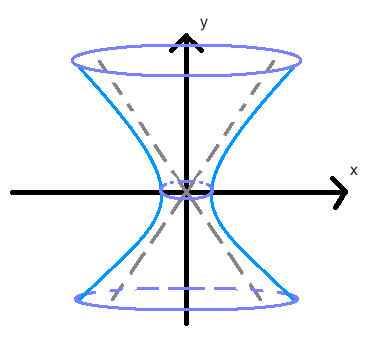
\includegraphics[width=0.5\textwidth]{images/dii.png}
\caption{$x^2-y^2=1$ rotated about the $y$-axis}
\label{dii figure}
\end{figure}

We see that geodesics travelling along the surface would diverge; hence this hyperboloid possesses negative curvature. A triangle on the surface would look like Figure \ref{neg curv triangle}, with the sum of its angles $< 180^{\circ}$.

\begin{figure}[h]
\centering
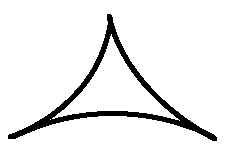
\includegraphics[width=0.3\textwidth]{images/negativeCurvTriangle.png}
\caption{Triangle with $\Sigma<180^{\circ}$}
\label{neg curv triangle}
\end{figure}

 %-----------------------------------------------------------

\begin{framed}
\textbf{iii.} The hyperbola $x^2-y^2=1$ is now rotated around the $x$-axis. What is the sign of the curvature this time? Why?
\end{framed}

\begin{figure}[h]
\centering
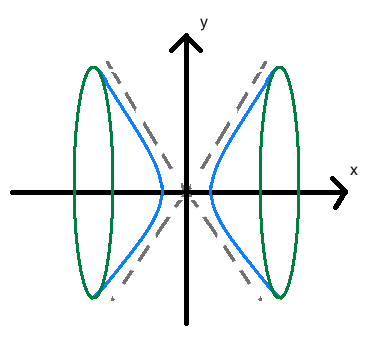
\includegraphics[width=0.5\textwidth]{images/diii.png}
\caption{$x^2-y^2=1$ rotated about the $x$-axis}
\label{diii figure}
\end{figure}

We see that geodesics travelling along the surface would converge; hence this hyperboloid possesses positive curvature. A triangle on the surface would look like Figure \ref{pos curv triangle} below, with the sum of its angles $> 180^{\circ}$.

\begin{figure}[h]
\centering
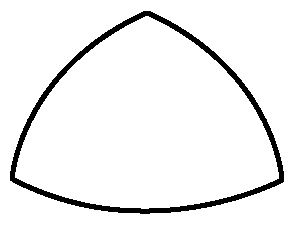
\includegraphics[width=0.3\textwidth]{images/positiveCurvTriangle.png}
\caption{Triangle with $\Sigma<180^{\circ}$}
\label{pos curv triangle}
\end{figure}


 %-----------------------------------------------------------

\begin{framed}
\textbf{iv.} Setting aside their dimensionality, in what fundamental way do the hyperboloids of revolution in parts (d)(ii) and (d)(iii) differ from Klein's geometry? Justify your answer in words; don’t try to calculate anything.
\end{framed}

The hyperboloids differ from Klein's geometry in that geodesics can ``traverse'' around the space and return to their origin (for example, by travelling on a geodesic around the hyperboloid). Further, for these hyperboloids we have non-constant curvature.

In the hyperboloid in Figure \ref{diii figure}, we note that there are obvious discontinuities. There are no discontinuities in Klein's geometry, which is an infinite plane.


 %-----------------------------------------------------------

\begin{framed}
\textbf{v.} Identify a spacetime manifold, that resembles Klein's geometry. Don’t worry too much about the precise mathematical meaning of ``resembles'', a qualitative justification is fine.
\end{framed}

We can consider anti-de Sitter space to resemble Klein's geometry. We would find that both have negative scalar curvature. The anti-de Sitter space is a maximally symmetric Lorenzian manifold (hence have a different signature metric), but ``locally'' the manifold would resemble Klein's geometry.

 %-----------------------------------------------------------

\begin{framed}
\textbf{(e)} Consider the triangle $\Delta$ABC, whose sides are ``straight lines'' (geodesics) joining the points A$(0,0)$, B$(b,0)$, and C$(0,b)$, with $b<1$. It is easy to show (you don't need to!) that the sides AB and AC are just the curves $v=0$ and $u=0$ respectively.
\end{framed}

\begin{framed}
\textbf{i.} What is the equation of the geodesic joining B and C?
\end{framed}

From Schutz (6.51), letting $\lambda$ be the parameter of the geodesic with $x^1=u$ and $x^2=v$ we have the geodesic equation
\begin{equation}
\frac{d}{d\lambda}\left(\frac{dx^{\alpha}}{d\lambda}\right)+\Gamma^{\alpha}_{\ph{\alpha}\mu\beta}
\frac{dx^{\mu}}{d\lambda}\frac{dx^{\beta}}{d\lambda}=0
\end{equation}
For $\alpha=1$ we have
\begin{align}
\frac{d}{d\lambda}\left(\frac{du}{d\lambda}\right)&=-\Gamma^{1}_{\ph{1}\mu\beta}
\frac{dx^{\mu}}{d\lambda}\frac{dx^{\beta}}{d\lambda}\\
&=-\Gamma^{1}_{\ph{1}11}\frac{dx^{1}}{d\lambda}\frac{dx^{1}}{d\lambda}
-\Gamma^{1}_{\ph{1}12}\frac{dx^{1}}{d\lambda}\frac{dx^{2}}{d\lambda}-
-\Gamma^{1}_{\ph{1}21}\frac{dx^{2}}{d\lambda}\frac{dx^{1}}{d\lambda}-
-\cancel{\Gamma^{1}_{\ph{1}22}\frac{dx^{2}}{d\lambda}\frac{dx^{2}}{d\lambda}}\\
&=-\Gamma^{1}_{\ph{1}11}\left(\frac{du}{d\lambda}\right)^2
-2\Gamma^{1}_{\ph{1}12}\frac{du}{d\lambda}\frac{dv}{d\lambda}
\end{align}
which can be written as
\begin{align}
\frac{d}{d\lambda}\left(\frac{du}{d\lambda}\right)+
\Gamma^{1}_{\ph{1}11}\left(\frac{du}{d\lambda}\right)^2
+2\Gamma^{1}_{\ph{1}12}\frac{du}{d\lambda}\frac{dv}{d\lambda}&=0\\
\Rightarrow \frac{d}{d\lambda}\left(\frac{du}{d\lambda}\right)+
2u(1-u^2-v^2)^{-1}\left(\frac{du}{d\lambda}\right)^2
+2v(1-u^2-v^2)^{-1}\frac{du}{d\lambda}\frac{dv}{d\lambda}&=0\label{geodes chris0}\\
\Rightarrow \frac{d}{d\lambda}\left(\frac{du}{d\lambda}\right)(1-u^2-v^2)^{-1}+
2u(1-u^2-v^2)^{-2}\left(\frac{du}{d\lambda}\right)^2
+2v(1-u^2-v^2)^{-2}\frac{du}{d\lambda}\frac{dv}{d\lambda}&=0\label{geodes chris1}\\
\Rightarrow \frac{d}{d\lambda}\left[(1-u^2-v^2)^{-1}\frac{du}{d\lambda}\right]&=0 \label{geodes chris2}
\end{align}

We shall prove that going from~(\ref{geodes chris1}) to~(\ref{geodes chris2}) is correct.
\begin{align}
\frac{d}{d\lambda}\left[(1-u^2-v^2)^{-1}\frac{du}{d\lambda}\right]&=
\frac{d}{d\lambda}\left[(1-u^2-v^2)^{-1}\right)\frac{du}{d\lambda}+(1-u^2-v^2)^{-1}\frac{d^2 u}{d\lambda^2}\\
&=\left[-\frac{d}{d\lambda}\left(-u^2\right)+-\frac{d}{d\lambda}\left(-v^2\right)\right]
(1-u^2-v^2)^{-2}\frac{du}{d\lambda}+(1-u^2-v^2)^{-1}\frac{d^2 u}{d\lambda^2}\\
&=\left[\frac{du}{d\lambda}\frac{d(u^2)}{du}+\frac{dv}{d\lambda}\frac{d(v^2)}{dv}\right]
(1-u^2-v^2)^{-2}\frac{du}{d\lambda}+(1-u^2-v^2)^{-1}\frac{d^2 u}{d\lambda^2}\\
&=\left[2u\frac{du}{d\lambda}+2v\frac{dv}{d\lambda}\right]
(1-u^2-v^2)^{-2}\frac{du}{d\lambda}+(1-u^2-v^2)^{-1}\frac{d^2 u}{d\lambda^2}\\
&=\text{LHS of}~(\ref{geodes chris1})
\end{align}

Hence this is indeed correct.

For $\alpha=2$ we have
\begin{align}
\frac{d}{d\lambda}\left(\frac{dv}{d\lambda}\right)&=-\Gamma^{2}_{\ph{1}\mu\beta}
\frac{dx^{\mu}}{d\lambda}\frac{dx^{\beta}}{d\lambda}\\
&=-\cancel{\Gamma^{2}_{\ph{2}11}\frac{dx^{1}}{d\lambda}\frac{dx^{1}}{d\lambda}}
-\Gamma^{2}_{\ph{2}12}\frac{dx^{1}}{d\lambda}\frac{dx^{2}}{d\lambda}-
-\Gamma^{2}_{\ph{2}21}\frac{dx^{2}}{d\lambda}\frac{dx^{1}}{d\lambda}-
-\Gamma^{2}_{\ph{2}22}\frac{dx^{2}}{d\lambda}\frac{dx^{2}}{d\lambda}\\
&=-\Gamma^{2}_{\ph{2}22}\left(\frac{dv}{d\lambda}\right)^2
-2\Gamma^{2}_{\ph{2}12}\frac{du}{d\lambda}\frac{dv}{d\lambda}\\
&=-2v(1-u^2-v^2)^{-1}\left(\frac{dv}{d\lambda}\right)^2
-2u(1-u^2-v^2)^{-1}\frac{du}{d\lambda}\frac{dv}{d\lambda}
\end{align}

By comparison with~(\ref{geodes chris0})-(\ref{geodes chris2}), we see that this implies
\begin{equation}
\frac{d}{d\lambda}\left[(1-u^2-v^2)^{-1}\frac{dv}{d\lambda}\right]=0
\end{equation}

We now find
\begin{align}
\frac{d}{d\lambda}\left[(1-u^2-v^2)^{-1}\frac{du}{d\lambda}\right]&=0\Rightarrow
(1-u^2-v^2)^{-1}\frac{du}{d\lambda}=c_1	\label{divide1}\\
\frac{d}{d\lambda}\left[(1-u^2-v^2)^{-1}\frac{dv}{d\lambda}\right]&=0\Rightarrow
(1-u^2-v^2)^{-1}\frac{dv}{d\lambda}=c_2	\label{divide2}
\end{align}

Dividing~(\ref{divide1}) by~(\ref{divide2}) we find
\begin{align}
\frac{du}{dv}&=\frac{c_1}{c_2}\equiv c_3\\
\Rightarrow v&=c_3 u+c_4
\end{align}

Since the point $(0,b)$ lies on the geodesic we have,
\begin{align}
b&=c_4\\
\Rightarrow c_4&=b
\intertext{Similarly using the point $(b,0)$,}
0&=bc_3+b\\
\Rightarrow c_3&=-1
\end{align}

Thus we conclude that equation of the geodesic joining $B$ and $C$ is
\begin{equation}
v=-u+b
\end{equation}

 %-----------------------------------------------------------

\begin{framed}
\textbf{ii.} Prove that the sum of the interior angles of $\Delta$ABC is
\begin{equation}
\Sigma = \angle\text{ABC}+\angle\text{BCA}+\angle\text{CAB}=\frac{\pi}{2}+2\cos^{-1}\left(\frac{1}{\sqrt{2-b^2}}\right).
\end{equation}
The sum of the angles is less than 180 degrees!
\end{framed}

The cosine of the angle between two vectors $\vec{M}$ and $\vec{N}$ is given by
\begin{equation}
\cos\theta=\frac{\vec{M}\cdot\vec{N}}{\lvert\vec{M}\rvert\lvert\vec{N}\rvert}
\end{equation}

In component notation we have
\begin{equation}
\theta=\cos^{-1}\left(\frac{g_{\alpha\beta}M^{\alpha}N^{\beta}}{\sqrt{g_{ij}M^{i}M^{j}g_{kl}N^{k}N^{l}}}\right)
\end{equation}

The angle between two curves at a point is equal to the angle between curves pointing in the same direction;

The equations bounding the triangle parametrised by $\lambda$ are given as
\begin{align}
\vec{a}&=(\lambda,0)\\
\vec{b}&=(0,\lambda)\\
\vec{c}&=(\lambda,b-\lambda)
\intertext{where $\lambda\leq b$.}
\Rightarrow \vec{\dot{a}}&=(1,0)\\
\vec{\dot{b}}&=(0,1)\\
\vec{\dot{c}}&=(1,-1)
\end{align}

We shall use these direction vectors WHY????.

\subsection*{Calculating $\angle$ABC}
We use $\vec{M}=\vec{\dot{a}}$ and $\vec{N}=\vec{\dot{c}}$. At the point B$(b,0)$,
\begin{align}
g_{11}&=\frac{a^2}{(1-b^2)^2}\\
g_{12}&=0\\
g_{22}&=\frac{a^2}{1-b^2}
\end{align}

Hence we find
\begin{align}
\angle\text{ABC}&=\cos^{-1}\left(\frac{g_{11}}{\sqrt{g_{11}g_{11}+g_{11}g_{22}}}\right)\\
&=\cos^{-1}\left(\frac{\frac{a^2}{(1-b^2)^{2}}}{\sqrt{\frac{a^4}{(1-b^2)^4}+\frac{a^4}{(1-b^2)^3}}}
\right)\\
&=\cos^{-1}\left(\frac{a^2}{(1-b^2)^2}\sqrt{\frac{1+(1-b^2)}{(1-b^2)^4}}\right)\\
&=\cos^{-1}\left(\frac{1}{\sqrt{2-b^2}}\right)
\end{align}

\subsection*{Calculating $\angle$BCA}
We use $\vec{M}=\vec{\dot{b}}$ and $\vec{N}=\vec{\dot{c}}$. At the point C$(0,b)$,
\begin{align}
g_{11}&=\frac{a^2}{1-b^2}\\
g_{12}&=0\\
g_{22}&=\frac{a^2}{(1-b^2)^2}
\end{align}

Hence we find
\begin{align}
\angle\text{BCA}&=\cos^{-1}\left(\frac{g_{22}}{\sqrt{g_{22}g_{11}+g_{22}g_{22}}}\right)\\
&=\cos^{-1}\left(\frac{\frac{a^2}{(1-b^2)^{2}}}{\sqrt{\frac{a^4}{(1-b^2)^4}+\frac{a^4}{(1-b^2)^3}}}
\right)\\
&=\cos^{-1}\left(\frac{a^2}{(1-b^2)^2}\sqrt{\frac{1+(1-b^2)}{(1-b^2)^4}}\right)\\
&=\cos^{-1}\left(\frac{1}{\sqrt{2-b^2}}\right)
\end{align}

\subsection*{Calculating $\angle$ABC}
We use $\vec{M}=\vec{\dot{a}}$ and $\vec{N}=\vec{\dot{c}}$. At the point B$(b,0)$,
\begin{align}
g_{11}&=\frac{a^2}{(1-b^2)^2}\\
g_{12}&=0\\
g_{22}&=\frac{a^2}{1-b^2}
\end{align}

Hence we find
\begin{align}
\angle\text{ABC}&=\cos^{-1}\left(\frac{g_{11}}{\sqrt{g_{11}g_{11}+g_{11}g_{22}}}\right)\\
&=\cos^{-1}\left(\frac{\frac{a^2}{(1-b^2)^{2}}}{\sqrt{\frac{a^4}{(1-b^2)^4}+\frac{a^4}{(1-b^2)^3}}}
\right)\\
&=\cos^{-1}\left(\frac{a^2}{(1-b^2)^2}\sqrt{\frac{1+(1-b^2)}{(1-b^2)^4}}\right)\\
&=\cos^{-1}\left(\frac{1}{\sqrt{2-b^2}}\right)
\end{align}


\subsection*{Calculating $\angle$CAB}
We use $\vec{M}=\vec{\dot{a}}$ and $\vec{N}=\vec{\dot{b}}$. At the point A$(0,0)$,
\begin{align}
g_{11}&=a^2\\
g_{12}&=0\\
g_{22}&=a^2
\end{align}

Hence we find
\begin{align}
\angle\text{BCA}&=\cos^{-1}\left(\frac{\cancel{g_{12}}}{\sqrt{g_{11}g_{22}}}\right)\\
&=\cos^{-1}\left(0\right)\\
&=\frac{\pi}{2}
\end{align}

Summing these angles we indeed find
\begin{equation}
\Sigma = \angle\text{ABC}+\angle\text{BCA}+\angle\text{CAB}=\frac{\pi}{2}+2\cos^{-1}\left(\frac{1}{\sqrt{2-b^2}}\right)
\end{equation}

as required.

 %-----------------------------------------------------------

\begin{framed}
\textbf{iii.} Triangles in Klein's geometry can have $\sum=0$! Without proof, sketch what such a triangle might look like. Your sketch by necessity will be an incomplete representation; there is no way to draw a Klein triangle faithfully on a flat page.
\end{framed}

A triangle in space with negative curvature will have $\Sigma<180^{\circ}$, as shown in Figure \ref{neg curv triangle}. One can imagine a triangle such as Figure \ref{no angle triangle} below.

\begin{figure}[h]
\centering
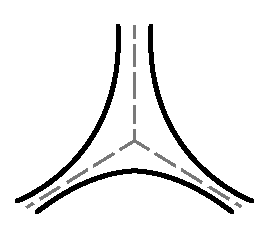
\includegraphics[width=0.3\textwidth]{images/zeroAngle.png}
\caption{Triangle with $\Sigma=0^{\circ}$}
\label{no angle triangle}
\end{figure}

If the dotted lines extended to infinity, we would have a triangle with $\Sigma=0^{\circ}$. In flat space, the lines would look somewhat parallel.

 %-----------------------------------------------------------

\begin{framed}
\textbf{(f) i.} Write down a closed form expression for the area A of $\Delta$ABC as an integral over a subset of the $(u,v)$ domain.
\end{framed}

Surface area depends not on the parameterisation of the space, but only on the surface itself. We have an expression for area
\begin{equation}
A=\int_{\text{surface}}\sqrt{\det g}~\text{d}A
\end{equation}

where $g$ is the metric. We have
\begin{align}
g&=\pmx{g_{11}&g_{12}\\g_{21}&g_{22}}\\
\Rightarrow \det g&=g_{11}g_{22}-g_{12}g_{21}\\
&=\frac{a^4(1-v^2)(1-u^2)-a^4 u^2 v^2}{(1-u^2-v^2)^4}\\
&=\frac{a^4}{(1-u^2-v^2)^4}\left[1-u^2-v^2+\cancel{u^2 v^2}-\cancel{u^2 v^2}\right]\\
&=\frac{a^4}{(1-u^2-v^2)^3}
\end{align}

We can now determine an expression for the area of $\Delta$ABC as
\begin{align}
A&=\iint \frac{a^4}{(1-u^2-v^2)^3}~\text{d}u~\text{d}v\\
&=\int_{v=0}^{v=b}\int_{u=0}^{u=b-v}\frac{a^2}{(1-u^2-v^2)^{3/2}}~\text{d}u~\text{d}v\label{abc area uv}
\end{align}

\begin{figure}[h]
\centering
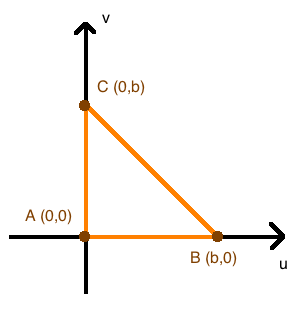
\includegraphics[width=0.5\textwidth]{images/fi.png}
\caption{The triangle $\Delta$ABC on the $u-v$ axis}
\label{fi figure}
\end{figure}


 %-----------------------------------------------------------

\begin{framed}
\textbf{ii.} By changing variables to $y=v+u$ and $z=v-u$, recast your integral in the form
\begin{equation}
A=2a^2\int^b_0 \frac{\text{d}y~y}{(2-y^2)\sqrt{1-y^2}}.
\end{equation}
Hence show that one has
\begin{equation}
A=a^2(\pi-\Sigma).\label{A(pi,Sigma)}
\end{equation}
\end{framed}

We begin by calculating the Jacobian,
\begin{align}
J(y,z)&=\pmx{\frac{\partial u}{\partial y}&\frac{\partial u}{\partial z}\\
\frac{\partial v}{\partial y}&\frac{\partial v}{\partial z}}=\pmx{\frac{1}{2}&-\frac{1}{2}\\\frac{1}{2}&\frac{1}{2}}\\
\Rightarrow \det J&=\frac{1}{2}
\end{align}

Next we consider the bounds of the integral; that is, the surface we are integrating over.
\begin{align}
(u,v)=(0,0)&\Rightarrow (y,z)=(0,0)\\
(u,v)=(b,0)&\Rightarrow (y,z)=(b,-b)\\
(u,v)=(0,b)&\Rightarrow (y,z)=(b,b)
\end{align}

\begin{figure}[h]
\centering
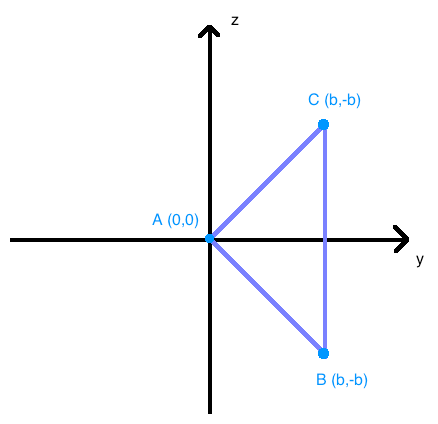
\includegraphics[width=0.5\textwidth]{images/fii.png}
\caption{The triangle $\Delta$ABC on the $y-z$ axis}
\label{yz figure}
\end{figure}

In $y-z$ space, our surface looks like Figure~\ref{yz figure} above. Just as we integrated over first $u$ in terms of $v$ then integrated over $v$ in~(\ref{abc area uv}), we shall integrate from $z=-y$ to $z=y$, then over $y=0$ to $y=b$.

Also note that we can express $u$ and $v$ in terms of $y$ and $z$ as
\begin{align}
u&=\frac{1}{2}(y-z)\\
v&=\frac{1}{2}(y+z)
\end{align}

Hence we can rewrite $A$ as
\begin{align}
A&=2a^2\int^{y=b}_{y=0}\int_{z=-y}^{z=y}\left(1-\left[\frac{1}{2}(y-z)\right]^2-\left[\frac{1}{2}(y+z)\right]^2\right)^{-3/2}\frac{1}{4}~\text{d}y~\text{d}z\\
&=\frac{a^2}{2}\int^{y=b}_{y=0}\int_{z=-y}^{z=y}
\left(1-\frac{1}{2}y^2-\frac{1}{2}z^2\right)^{-3/2}~\text{d}y~\text{d}z
\intertext{We now let $m=1-\frac{1}{2}y^2$, and let $z=\sqrt{2m}\sin r \Rightarrow \text{d}z=\sqrt{2m}\cos r~\text{d}r$}
A&=\frac{a^2}{2}\int^{y=b}_{y=0}\int^{r=\sin^{-1}\left(\frac{y}{\sqrt{2m}}\right)}
_{r=-\sin^{-1}\left(\frac{y}{\sqrt{2m}}\right)}
\left(\underbrace{m-m\sin^2 r}_{=m(\cos^2 r)}\right)^{-3/2}~\text{d}y~\sqrt{2m}\cos r~\text{d}r\\
&=\frac{a^2}{2}\iint
\sqrt{2}m^{-1}\cos^{-2}r~\text{d}y~\text{d}r\\
&=\frac{a^2}{\sqrt{2}}\int^{y=b}_{y=0}m^{-1}\bigg[\tan(r)\bigg]
^{\sin^{-1}\left(\frac{y}{\sqrt{2m}}\right)}_{-\sin^{-1}\left(\frac{y}{\sqrt{2m}}\right)}
~\text{d}y\label{some eq1}\\
&=\frac{a^2}{\sqrt{2}}\int m^{-1}\left[\frac{2y}{\sqrt{2-2y^2}}\right]~\text{d}y\label{some eq2}
\end{align}
In moving from~(\ref{some eq1}) to~(\ref{some eq2}) we use the identity
\begin{align}
\tan\left[\sin^{-1}(ax)\right]&=\frac{ax}{\sqrt{1-a^2x^2}}\\
\Rightarrow \tan\left[\sin^{-1}\left(\frac{y}{\sqrt{2m}}\right)\right]
&=\frac{\frac{y}{\sqrt{2m}}}{\sqrt{1-\frac{y^2}{2m}}}\\
&=\frac{y}{\sqrt{2m-y^2}}
\intertext{Since $m=1-\frac{1}{2}y^2$ we find}
\tan\left[\sin^{-1}\left(\frac{y}{\sqrt{2m}}\right)\right]&=\frac{y}{\sqrt{2-2y}}
\end{align}

Continuing from~(\ref{some eq2}),
\begin{align}
A&=\frac{a^2}{\sqrt{2}}\int^{b}_{0} m^{-1}\left[\frac{2y}{\sqrt{2-2y^2}}\right]~\text{d}y\\
&=a^2\int^{b}_{0}\frac{1}{1-\frac{1}{2}y^2}\frac{y}{\sqrt{1-y^2}}~\text{d}y\\
&=2a^2\int^{b}_{0}\frac{\text{d}y~y}{(2-y^2)\sqrt{1-y^2}}
\end{align}

as required.

We will now show that $A=a^2(\pi-\Sigma)$.

\begin{align}
A&=2a^2\int^b_0 \frac{\text{d}y~y}{(2-y^2)\sqrt{1-y^2}}
\intertext{Let $p=\sqrt{1-y^2}$}
\Rightarrow \frac{dp}{dy}&=\frac{-2y\times\frac{1}{2}}{\sqrt{1-y^2}}=-\frac{y}{\sqrt{1-y^2}}
=-\frac{y}{p}\\
\Rightarrow A&=2a^2\int^{p=\sqrt{1-b^2}}_{p=1}\frac{1}{1+p^2}\frac{1}{p}y\times
\frac{-p}{y}~\text{d}p\\
&=-2a^2\int^{\sqrt{1-b^2}}_{1}\frac{1}{1+p^2}~\text{d}p\\
&=2a^2\int_{\sqrt{1-b^2}}^{1}\frac{1}{1+p^2}~\text{d}p\\
&=2a^2\left[\tan^{-1}(p)\right]^{1}_{\sqrt{1-b^2}}\\
&=2a^2\left[\tan^{-1}(1)-\tan^{-1}\left(\sqrt{1-b^2}\right)\right]\\
&=2a^2\left[\frac{\pi}{4}-\tan^{-1}\left(\sqrt{1-b^2}\right)\right]\label{pi sigma pre}
\intertext{We now consider the remaining $\tan^{-1}$ term.}
\tan^{-1}(x)&=\sin^{-1}\left(\frac{x}{\sqrt{x^2+1}}\right)\\
\Rightarrow \tan^{-1}\left(\sqrt{1-b^2}\right)&=
\sin^{-1}\left(\frac{\sqrt{1-b^2}}{\sqrt{2-b^2}}\right)\\
&=\sin^{-1}\left(\sqrt{\frac{2-b^2-1}{2-b^2}}\right)\\
&=\sin^{-1}\left(\sqrt{1-\frac{1}{2-b^2}}\right)\\
\cos^{-1}(x)&=\sin^{-1}\left(\sqrt{1-x^2}\right),\quad\text{if }0 \leq x \leq 1\\
\Rightarrow \tan^{-1}\left(\sqrt{1-b^2}\right)&= \sin^{-1}\left(\sqrt{1-\frac{1}{2-b^2}}\right)=
\cos^{-1}\left(\frac{1}{\sqrt{2-b^2}}\right)
\intertext{Substituting this into~(\ref{pi sigma pre}) we conclude}
A&= 2a^2\left[\frac{\pi}{4}-\cos^{-1}\left(\frac{1}{\sqrt{2-b^2}}\right)\right]\\
&=a^2\left[\frac{\pi}{2}-2cos^{-1}\left(\frac{1}{\sqrt{2-b^2}}\right)\right]\\
&=a^2\left(\frac{\pi}{2}-\Sigma\right)
\end{align}
as required. 
 
 
 %-----------------------------------------------------------

\begin{framed}
\textbf{iii.} Explain briefly, in one or two sentences, why~(\ref{A(pi,Sigma)}) guarantees the \emph{nonexistence} of similar triangles in Klein’s geometry.
\end{framed}

The equation
\begin{equation*}
A=a^2\left(\frac{\pi}{2}-\Sigma\right)
\end{equation*}
tells us that in Klein's geometry, the area of a triangle is linked directly to the sum of its internal angles. Similar triangles possess the same internal angles and hence the same sum of internal angles; however since equation~(\ref{A(pi,Sigma)}) gives only a single value of area for any $\Sigma$, we see that the area is fixed, and hence similar triangles cannot exist in Klein's geometry.

 %-----------------------------------------------------------

\begin{framed}
\textbf{(g)} A vector $\vec{W}$ with equal components $W^1$ and $W^2$ at the point $A(0,0)$ is parallel transported along the geodesic AB. Show that its components, when it reaches the point B$(b,0)$, are in the ratio
\begin{equation}
\frac{W^1}{W^2}=(1-b^2)^{1/2}
\end{equation}
\end{framed}

Parallel transport of a vector $\vec{V}$ along a curve $s$ is given by
\begin{equation}
U^{\beta}V^{\alpha}_{\ph{\alpha};\beta}=0
\end{equation}

As $V$ does not change ove the geodesic $AB$, we know $x^{\beta}=u=x^{1}$.

We have two geodesic equations for the transport of $\vec{W}$ along $AB$:

\begin{align}
\frac{\partial W^{1}}{\partial u}+\Gamma^{1}_{\ph{1}11}W^{1}
+\Gamma^{1}_{ph{1}21}W^2&=0 \label{W1 diff eqn}\\
\frac{\partial W^{2}}{\partial u}+\Gamma^{2}_{\ph{2}21}W^2&=0
\end{align}

Solving the second equation gives us
\begin{align}
\frac{\partial W^2}{\partial u}+\frac{u}{1-u^2-v^2}W^2&=0\\
\Rightarrow \frac{\text{d}W^2}{W^2}&=-\frac{u~\text{d}u}{1-u^2-v^2}\\
\log W^2&=\frac{1}{2}\log(1-u^2-v^2)+c_{1}\\
W^2&=c_1\sqrt{1-u^2-v^2}\label{W2 eqn}
\end{align}

Now, substituting~(\ref{W2 eqn}) into~(\ref{W1 diff eqn}) we find
\begin{align}
\frac{\partial W^{1}}{\partial u}+\frac{2u}{1-u^2-v^2}W^1=\frac{c_1 v	}{\sqrt{1-u^2-v^2}}&=0\\
(1-u^2-v^2)^{-1}\frac{\text{d}W^{1}}{\text{d}u}+\frac{2u}{(1-u^2-v^2)^2} W^{1}
+\frac{c_1 v}{(1-u^2-v^2)^{3/2}}&=0\\
\frac{\partial}{\partial u}\left(\frac{W^{1}}{1-u^2-v^2}\right)&=-\frac{c_1 v}{(1-u^2-v^2)^{3/2}}\\
\frac{W^1}{1-u^2-v^2}&=-c_1\int \frac{v~\text{d}v}{(1-u^2-v^2)^{3/2}}
\end{align}

We shall solve this integral through some clever substitution. We let
\begin{align}
k&=1-v^2,\\
m&=\sqrt{k}\sin n
\end{align}

Then, we have
\begin{align}
\Rightarrow \int\frac{v~\text{d}v}{(1-u^2-v^2)^{3/2}}&=\frac{1}{(k-u^2)^{3/2}}\\
&=k^{-3/2}\int \sec^2 n ~ \text{d}n\\
&=k^{-3/2}\tan n + c_2\\
&=k^{-3/2}\frac{n}{\sqrt{k^2-n^2}}+c_2\\
&=\left(1-v^2)\right)^{-3/2}\frac{u}{\sqrt{1-u^2-v^2}}+c_2
\end{align}

So now we have
\begin{align}
\left(1-u^2-v^2\right)^{-1}W^{1}&=-c_1\left(1-v^2\right)^{-3/2}\frac{vu}{\sqrt{1-u^2-v^2}}+c_3\\
\Rightarrow W^{1}&=-c_1 \left(1-v^2\right)^{-3/2}vu\sqrt{1-u^2-v^2}+c_3\left(1-u^2-v^2\right)
\label{W1 eqn}
\end{align}

We can now combine~(\ref{W1 eqn}) and ~(\ref{W2 eqn}) to find the ratio $\frac{W^1}{W^2}$.

At $(u,v)=(0,0)$, we have $\vec{W}=(w,w)$ (where $w$ is some constant; the components are equal at this point) so
\begin{align}
W^1(0,0)&=w=c_3\\
W^2(0,0)&=w=c_1
\end{align}

Considering the point $(u,v)=(b,0)$ we find
\begin{align}
\frac{W^1}{W^2}&=\frac{c_3}{(1-b^2)}{c\sqrt{1-b^2}}\\
&=\frac{w}{w}\left(1-b^2\right)^{-1/2}\\
&=\left(1-b^2\right)^{-1/2}
\end{align}

as required.

\end{document}







































